\section{Risk Assessment}
\subsection{Risk Assessment Risk Matrix}

\begin{longtable}[h!]{ | p{2.25cm} | p{2.25cm} | p{2.25cm} | p{2.25cm} | p{2.25cm} | p{2.25cm} | }\hline
& \multicolumn{5}{|c|}{\textbf{Consequences}}\\\hline
\textbf{Likelihood} & \textbf{Catastrophic (Cat)} & \textbf{Major (Maj)} & \textbf{Moderate (Mod)} & \textbf{Minor (Min)} & \textbf{Insignificant (Ins)} \\\hline
\textbf{Almost Certain (AC)} & \cellcolor{red}\textbf{Very High (VH)} & \cellcolor{red}\textbf{Very High (VH)} & \cellcolor{orange}\textbf{High (H)} & \cellcolor{yellow}\textbf{Medium (M)} & \cellcolor{green}\textbf{Very Low (VL)} \\\hline
\textbf{Likely (L)} & \cellcolor{red}\textbf{Very High (VH)} & \cellcolor{orange}\textbf{High (H)} & \cellcolor{yellow}\textbf{Medium (M)} & \cellcolor{lime}\textbf{Low (L)} & \cellcolor{green}\textbf{Very Low (VL)} \\\hline
\textbf{Possible (P)} & \cellcolor{orange}\textbf{High (H)} & \cellcolor{orange}\textbf{High (H)} & \cellcolor{yellow}\textbf{Medium (M)} & \cellcolor{lime}\textbf{Low (L)} & \cellcolor{green}\textbf{Very Low (VL)} \\\hline
\textbf{Unlikely (U)} & \cellcolor{yellow}\textbf{Medium (M)} & \cellcolor{yellow}\textbf{Medium (M)} & \cellcolor{lime}\textbf{Low (L)} & \cellcolor{green}\textbf{Very Low (VL)} & \cellcolor{green}\textbf{Very Low (VL)} \\\hline 
\textbf{Rare (R)} & \cellcolor{lime}\textbf{Low (L)} & \cellcolor{lime}\textbf{Low (L)} & \cellcolor{lime}\textbf{Low (L)} & \cellcolor{green}\textbf{Very Low (VL)} & \cellcolor{green}\textbf{Very Low (VL)} \\\hline
\caption{Risk Assessment Matrix}
\label{tab:RiskMatrix}
\end{longtable}

\begin{longtable}{ | P{3cm } | P{7cm} | }
\hline
\textbf{Risk Level}& \textbf{What should I do?} \\
\hline
\cellcolor{red}\textbf{Extreme}& Eliminate from activities \\
\hline
\cellcolor{orange}\textbf{High}& Eliminate from activities \\ 
\hline
\cellcolor{yellow}\textbf{Medium}& Specific monitoring or procedures required, management responsibility must be specified \\
\hline
\cellcolor{green}\textbf{Low}& Manage through routine procedures. Unlikely to need specific application of resources \\
\hline
\caption{Risk Level Management}
\label{tab:RiskManagement}
\end{longtable}

\clearpage
\subsection{Identified Risks} 

\begin{comment}
In table \ref{tab:RiskID}, (C) are consequences, (L) is likelihood and (LvL) is the level of risk.

\begin{longtable}{ | P{3.75cm} | P{3.5cm} | P{0.7cm} |  P{0.5cm} |  P{1cm} | P{3.75cm} | }
\hline
\textbf{What could cause harm?}& \textbf{What could go wrong?}& \textbf{C}& \textbf{L}& \textbf{LvL}& \textbf{What controls are required?} \\
\hline
Actively handling sensitive electronics& Risk of destroying components with ESD& \cellcolor{green}Ins& \cellcolor{green}R& \cellcolor{green}VL& Wear ESD wristband when handling sensitive electronics. \\
\hline
Soldering electronic connections& Burns and inhalation of solder fumes& \cellcolor{green}I& \cellcolor{green}R& \cellcolor{green}VL& Safety glasses and gloves. Extractor fans / ventilation. \\
\hline
Placing equipment on a tall footbridge over a busy highway& Dropping equipment onto the traffic below and causing an accident& \cellcolor{green}M& \cellcolor{green}U& \cellcolor{green}VL& Bridge has protective railing. Design a lightweight system and gain supervisor approval before field implementation. \\
\hline
Vibrating beam experiment& Crushing or physical injury& \cellcolor{green}I& \cellcolor{green}R& \cellcolor{green}VL& Wear enclosed footwear. Ensure surroundings are clear. Keep distance whilst experiment is running. \\
\hline
\caption{Identified Risks}
\label{tab:RiskID} 
\end{longtable}
\end{comment}

\begin{figure}[h!]
\centering
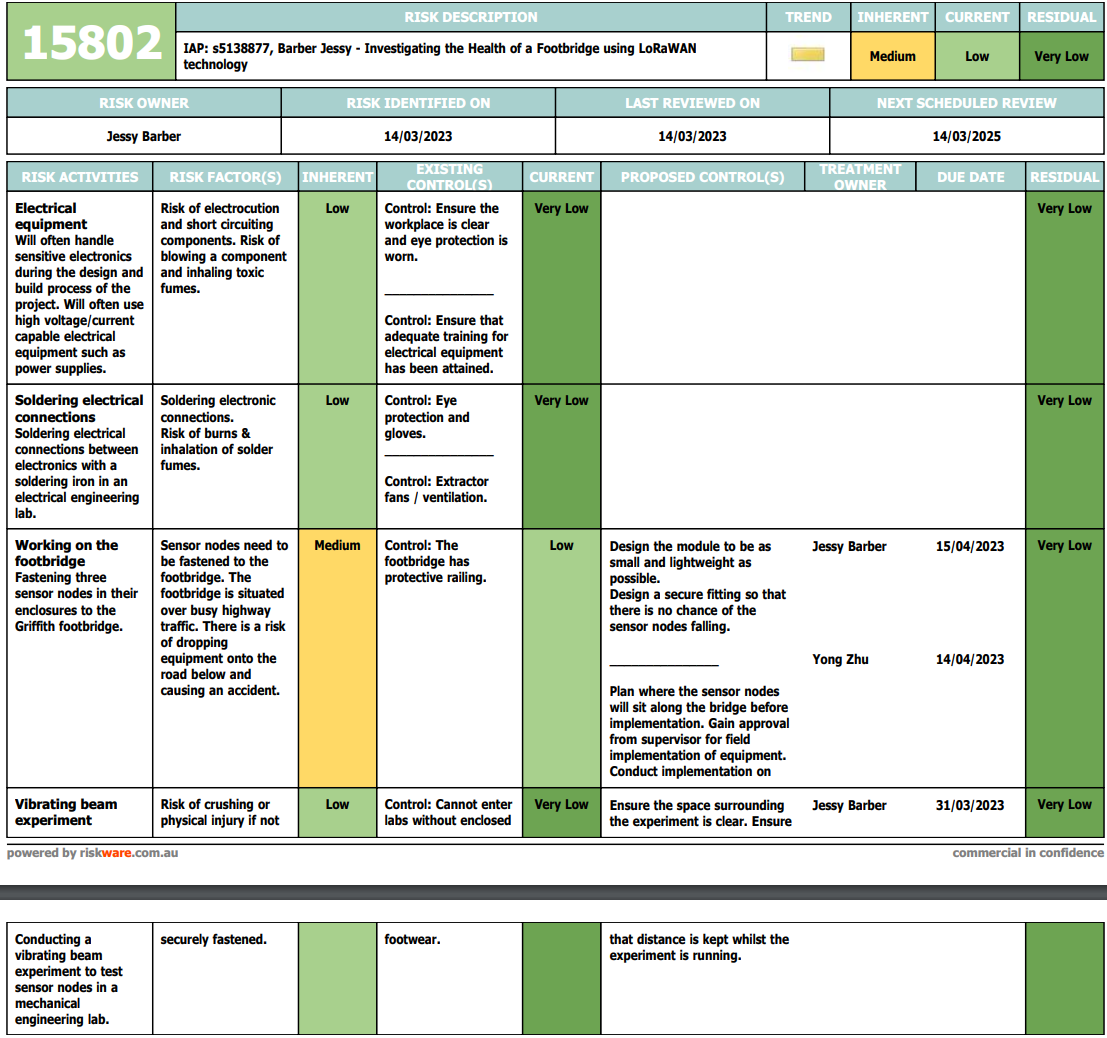
\includegraphics[scale=0.6,angle=90,origin=c]{Images/Risks.png}
\caption{GSAFE Risk Assessment}
\label{fig:GSAFE}
\end{figure}



